\documentclass[a4paper,10pt,headlines=3.2]{scrartcl}
\usepackage{graphicx}           %Bilder

%\usepackage[T1]{fontenc}        %Umlaute
%\usepackage[latin1]{inputenc}   %Windows
%\usepackage[utf8x]{inputenc}	%Linux
\usepackage{ucs}

\usepackage[ngerman]{babel}     %Deutsche Sprache
\usepackage{amsmath}            %Math. Zeichen
\usepackage{pifont}             %Skalierbare Schriftart
\usepackage{array}
\usepackage{epsfig}             %Erweiterte Grafiken
\usepackage{makeidx}            %Stichwortverzeichnis
\usepackage[pdftex]{color} 

\newcommand{\changefont}[3]{
\fontfamily{#1} \fontseries{#2} \fontshape{#3} \selectfont}

\makeindex

\usepackage[automark]{scrpage2}
\usepackage[nosectionbib]{apacite}               %Zitieren

%\usepackage[colorlinks]{hyperref}%Hyperlinks

\usepackage{lmodern}
\usepackage{scrpage2}           %KOMA-Script
\usepackage{tipa}
\usepackage{qtree}
\usepackage{pgf}


\usepackage{remreset}			%Fussnoten global
\makeatletter
\@removefromreset{footnote}{chapter}
\makeatother 

\setcounter{tocdepth}{3}

%Kopfzeilen
\pagestyle{scrheadings}         %Seitenstil scrheadings verwenden

%\setlength{\textheight}{24cm}
%\setlength{\textwidth}{16cm}
%\setlength{\topmargin}{-2cm}
%\setlength{\oddsidemargin}{0cm}

% Groesse des Textbereiches in der Seite
\setlength{\textwidth}{16cm}
\setlength{\textheight}{22cm}
% Kopf- und Fusszeile, Hoehe und Abstand vom Text
\setlength{\headheight}{15pt}
\setlength{\headsep}{0.8cm}
% Linker Seiteneinzug
\setlength{\oddsidemargin}{2.5cm} \addtolength{\oddsidemargin}{-1in}
\setlength{\evensidemargin}{2.5cm} \addtolength{\evensidemargin}{-1in}
% Andere Groessen ausrechnen (vertikal zentrieren)
\setlength{\footskip}{\headsep}
\addtolength{\footskip}{\headheight}
\setlength{\topmargin}{\paperheight}
\addtolength{\topmargin}{-\textheight}
\addtolength{\topmargin}{-\headheight}
\addtolength{\topmargin}{-\headsep}
\addtolength{\topmargin}{-\footskip}
\addtolength{\topmargin}{-2in}
\addtolength{\topmargin}{-0.5\topmargin}

%Schriftart
\changefont{cmss}{m}{n}

%Abstand zur�cksetzen
\setlength{\headheight}{20pt}

\usepackage{listings} 
\lstset{numbers=left, numberstyle=\tiny, numbersep=5pt} \lstset{language=Java} 

\clearscrheadfoot
%\renewcommand{\headheight}{40pt} 
\ihead[]{Datenstrukturen und Algorithmen \\Fr�hlingssemester 2011 \\Institut f�r angewandte Mathematik} % - links
\ohead[asdasd]{�bungsblatt 5 \\Abgabetermin 31. M�rz 2011 \\Adrianus Kleemans [07-111-693]} % - linke Kopfzeile 
\setheadsepline{.4pt} %Separate Linie im Kopf
\cfoot[\pagemark]{\pagemark} %- mittlere Fusszeile 

\begin{document}
\section*{Theoretische Aufgaben}
\subsection*{Aufgabe 1}
\lstset{frame=single}
\begin{lstlisting}[caption=Aufgabe 1]{Name}
reverse(list l)
//falls Liste 0 oder 1 Element enth�lt
if list.size <= 1
  return l

// Schleife startet mit zweitem Element der Liste.
// 'next' ist der Zeiger auf das n�chste Feld, 
// die Funktion zeigeAuf() ermittelt die Adresse des Elements.
for i=1 to l.size
    l[i].next = zeigeAuf(l[i-1])

return l
\end{lstlisting}

\subsection*{Aufgabe 2}
\begin{lstlisting}[caption=Aufgabe 2]{Name}
void enqueue(element e)
//Wir brauchen 'tail', um in linearer Zeit Elemente hinzuf�gen zu k�nnen. 
//Da die Listenelemente gem�ss Aufgabe nebst 'key' nur das Feld 'next' 
//besitzt, wird dieses verwendet, um auf das vorherige Element zu zeigen.

//Zeiger des neuen Elements auf NULL setzen
e.next = NULL

//Element vor tail soll auf e zeigen
(tail.next).next = zeigeAuf(e)

//tail soll auf e zeigen
tail.next = zeigeAuf(e)
----------------------------------------------------------------------------
element dequeue()
//Wenn Liste leer, NULL zur�ckgeben und nichts ver�ndern
if tail.next = head
  return NULL

element k = head.next
head.next = zeigeAuf((head.next).next)

//Wenn letztes vorhandenes Element entfernt werden soll:
//Durch obere Anweisung wurde head.next bereits auf NULL
//gesetzt. Nun muss noch tail auf head zeigen:
if head.next = NULL
  tail.next = zeigeAuf(head)

return k
\end{lstlisting}
\texttt{Start}: \{(head) $\leftarrow$ (tail)\}\\
\texttt{ENQUEUE(3)}: \{(head) $\rightarrow$ 3 $\leftarrow$ (tail)\}\\
\texttt{ENQUEUE(5)}: \{(head) $\rightarrow$ 3 $\rightarrow$ 5 $\leftarrow$ (tail)\}\\
\texttt{DEQUEUE()}: \{(head) $\rightarrow$ 5 $\leftarrow$ (tail)\}, return 3\\
\texttt{ENQUEUE(2)}: \{(head) $\rightarrow$ 5 $\rightarrow$ 2 $\leftarrow$ (tail)\}\\
\texttt{DEQUEUE()}: \{(head) $\rightarrow$ 2 $\leftarrow$ (tail)\}, return 5\\
\texttt{ENQUEUE(8)}: \{(head) $\rightarrow$ 2 $\rightarrow$ 8 $\leftarrow$ (tail)\}\\
\texttt{ENQUEUE(9)}: \{(head) $\rightarrow$ 2 $\rightarrow$ 8 $\rightarrow$ 9 $\leftarrow$ (tail)\}\\
\texttt{DEQUEUE()}: \{(head) $\rightarrow$ 8 $\rightarrow$ 9 $\leftarrow$ (tail)\}, return 2\\
\texttt{DEQUEUE()}: \{(head) $\rightarrow$ 9 $\leftarrow$ (tail)\}, return 8\\
\texttt{DEQUEUE()}: \{(head) $\leftarrow$ (tail)\}, return 9\\
\texttt{DEQUEUE()}: \{(head) $\leftarrow$ (tail)\}, return NULL\\
\texttt{Ende}: \{(head) $\leftarrow$ (tail)\}\\

\subsection*{Aufgabe 3}
\begin{lstlisting}[caption=Aufgabe 3]{Name}
output(node n)
print n.key
if n.left-child != NULL
  output(n.left-child)
if n.right-sibling != NULL
  output(n.right-sibling)
\end{lstlisting}

\subsection*{Aufgabe 4}
\begin{lstlisting}[caption=Aufgabe 4]{Name}
output(node n)

while stack != empty
  print n
  if n.left-child != NULL
    stack.push(n.left-child)
  if n.right-sibling != NULL
    stack.push(n.right-sibling)
  n=stack.pop

\end{lstlisting}


\section*{Praktische Aufgaben}
\subsection*{Aufgabe 1}
Siehe Anhang \texttt{KDTreeVisualization.java}.
\subsection*{Aufgabe 2}
Siehe Anhang \texttt{KDTreeVisualization.java}.\\
Ausgabe \textit{Visualize KD Tree}:
\begin{figure}[ht]
\centering
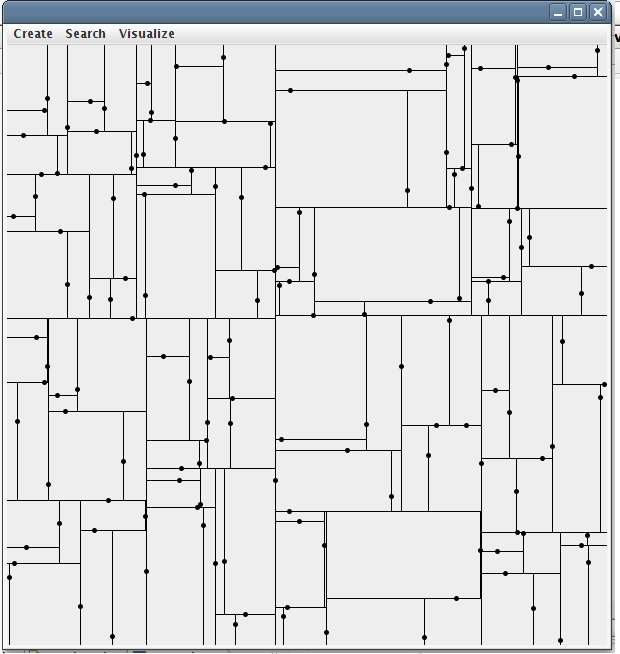
\includegraphics[height=8cm]{kdtree}
\end{figure}
\subsection*{Aufgabe 3}
\begin{figure}[ht]
\centering
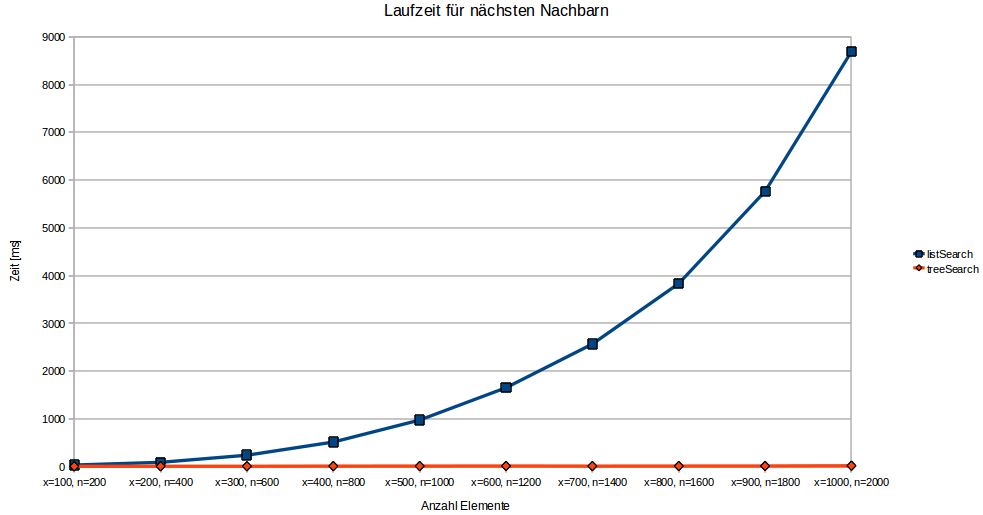
\includegraphics[height=8cm]{graph3}
\end{figure}
\begin{center}
\begin{tabular}{|l|c|c|}\hline
\textbf{Parameter} & \textbf{listSearch} & \textbf{treeSearch}\\\hline
x=100, n=200 & 36ms & 8ms\\\hline
x=200, n=400 & 92ms & 11ms\\\hline
x=300, n=600 & 241ms & 10ms\\\hline
x=400, n=800 & 517ms & 13ms\\\hline
x=500, n=1000 & 977ms & 14ms\\\hline
x=600, n=1200 & 1655ms & 16ms\\\hline
x=700, n=1400 & 2569ms & 13ms\\\hline
x=800, n=1600 & 3836ms & 15ms\\\hline
x=900, n=1800 & 5766ms & 16ms\\\hline
x=1000, n=2000 & 8693ms & 21ms\\\hline
\end{tabular}
\end{center}
Da die beiden Faktoren x und n, respektive Gesamtanzahl Punkt und zu suchende Punkte einander beinflussen, kann keine
genaue Vorhersage getroffen werden. Die Grafik l�sst aber vermuten, dass sich die beiden Laufzeitfunktionen $\Theta(n)$
resp. $\Theta(log(n))$ ann�hern.

\end{document}